%============================== Setting teh Document=============================================

\documentclass{beamer}
\usepackage[italian]{babel} 
\usepackage[latin1]{inputenc} 
\usepackage[T1]{fontenc}
\usepackage{graphicx} 
\usetheme{Madrid} 


%==========================Set the foot line========================================================
%-> Set the foot line.
\makeatletter
\setbeamertemplate{footline}
{
  \leavevmode%
\hbox{%
	\begin{beamercolorbox}[wd=.333333\paperwidth,ht=2.25ex,dp=1ex,center]{author in head/foot}%
	\usebeamerfont{author in head/foot}\insertsection
\end{beamercolorbox}%
\begin{beamercolorbox}[wd=.333333\paperwidth,ht=2.25ex,dp=1ex,center]{title in head/foot}%
	\usebeamerfont{title in head/foot}\insertsubsection
\end{beamercolorbox}%
\begin{beamercolorbox}[wd=.333333\paperwidth,ht=2.25ex,dp=1ex,right]{date in head/foot}%
	\usebeamerfont{date in head/foot}\insertshortdate{}\hspace*{2em}
	\insertframenumber{} / \inserttotalframenumber\hspace*{2ex} 
\end{beamercolorbox}}%
}%
\vskip0pt%

\makeatother



\title{Analisi della struttura sanitaria della provincia di Ascoli Piceno} 
\author{Enrico Ferretti \\ 
	Tommaso Cicco\\
	Francesco Rombaldoni\\
	} 
\institute{Universit� degli Studi di Urbino "Carlo Bo"} 
\logo{\includegraphics[width=15mm]{Uni}}


%\usetheme{AnnArbor}

%\useoutertheme[right]{sidebar} 
\setbeamercovered{dynamic}

%=========================================== Starting Document=====================================
\begin{document}

%Prima slide (Copertina)
\section{Test Section One}
\subsection{Test Subsection One One}

	\begin{frame} 
		\maketitle 		
	\end{frame}

	\begin{frame} 
		\frametitle{Indice} 
		\tableofcontents 
	\end{frame}


	\section{Presentazione}
	\begin{frame} 
		\frametitle{Obbiettivo:} 
	%	\framesubtitle{Sottotitolo} 
	L'obbiettivo dell'analisi � di determinare se la rete delle strutture della provincia di Ascoli Piceno che erogano servizi d'assistenza psichiatrica corrisponde a una delle seguenti strutture ed il cambiamento negli anni 2015, 2017, 2019:  
	
	\bigskip
	
	\begin{enumerate}
		\item Organizzazione diffusa.
		\item Organizzazione centralizzata.
		\item Organizzazione Integrata
	\end{enumerate}

\end{frame}

%----------------------Staring report part-----------------------------

\section{Operazioni Svolte}

\begin{frame}
	\frametitle{Operazioni svolte}
	I grafi, che rappresentano la struttura della rete, sono stati generati tramite il software Gephi; sono state inoltre svolte le seguenti operazioni:
	
	\bigskip
	
	\begin{enumerate}
		\item Determinazione della centralit� relativa alla closeness.
		\item Calcolo della centralizzazione dei grafi.
		\item Determinazione del K-core.
	\end{enumerate}
\end{frame}

\section{Anno 2015}

\begin{frame}
	\frametitle{Anno 2015}
	\framesubtitle{Statistiche generali}
	\begin{itemize}
		\item Rete formata da 25 nodi e 79 archi.
		\item Il nodo pi� centrale � "CSM Ospedale AP".
		\item Centralizzazione del grafo: 0,49.
		\item Unica componente connessa.
	\end{itemize} 
\end{frame}

\begin{frame}
	\frametitle{Anno 2015}
	\framesubtitle{Centralit�}
	\begin{figure}
		\centering
		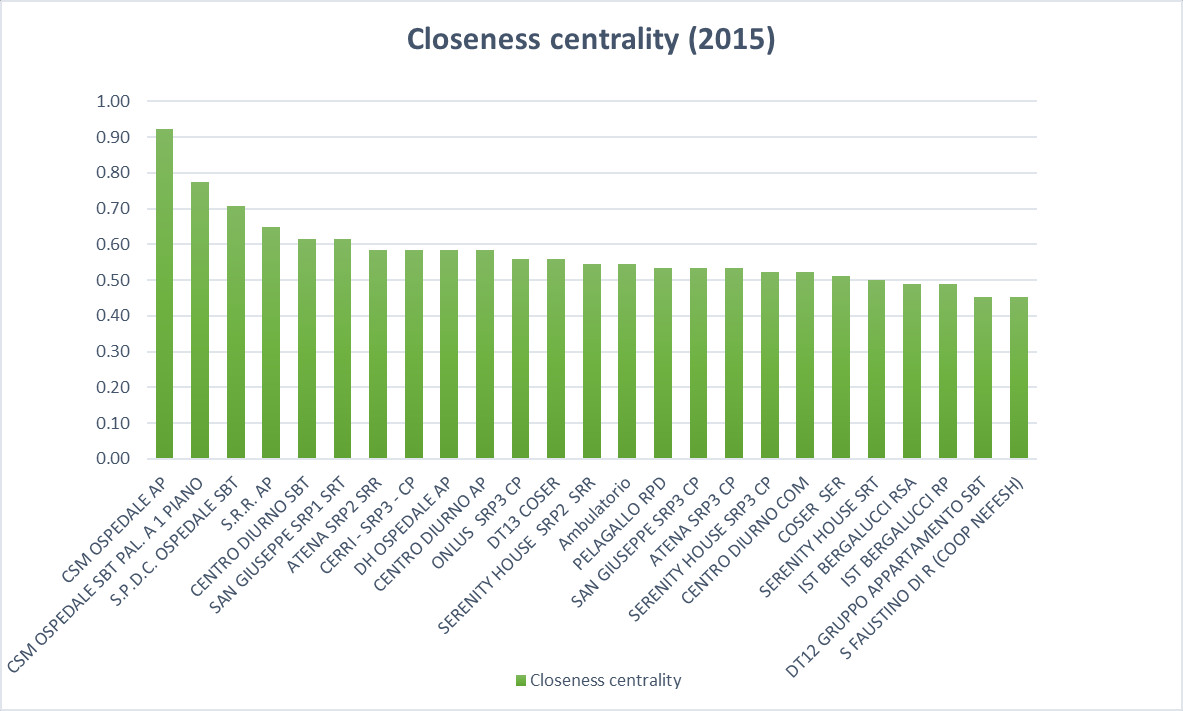
\includegraphics[width=0.8\linewidth]{imgs/2015_diagram}
		\label{fig:2015diagram}
	\end{figure}
\end{frame}

\section{Anno 2017}
\begin{frame}
	\frametitle{Anno 2017}
	\framesubtitle{Statistiche generali}
	\begin{itemize}
		\item Rete formata da 31 nodi e 94 archi.
		\item Il nodo pi� centrale � "CSM Ospedale AP".
		\item Centralizzazione del grafo: 0,38.
		\item Nodo isolato: "Atena SRP3 CP". 
	\end{itemize} 
\end{frame}

\begin{frame}
	\frametitle{Anno 2017}
	\framesubtitle{Centralit�}
	\begin{figure}
		\centering
		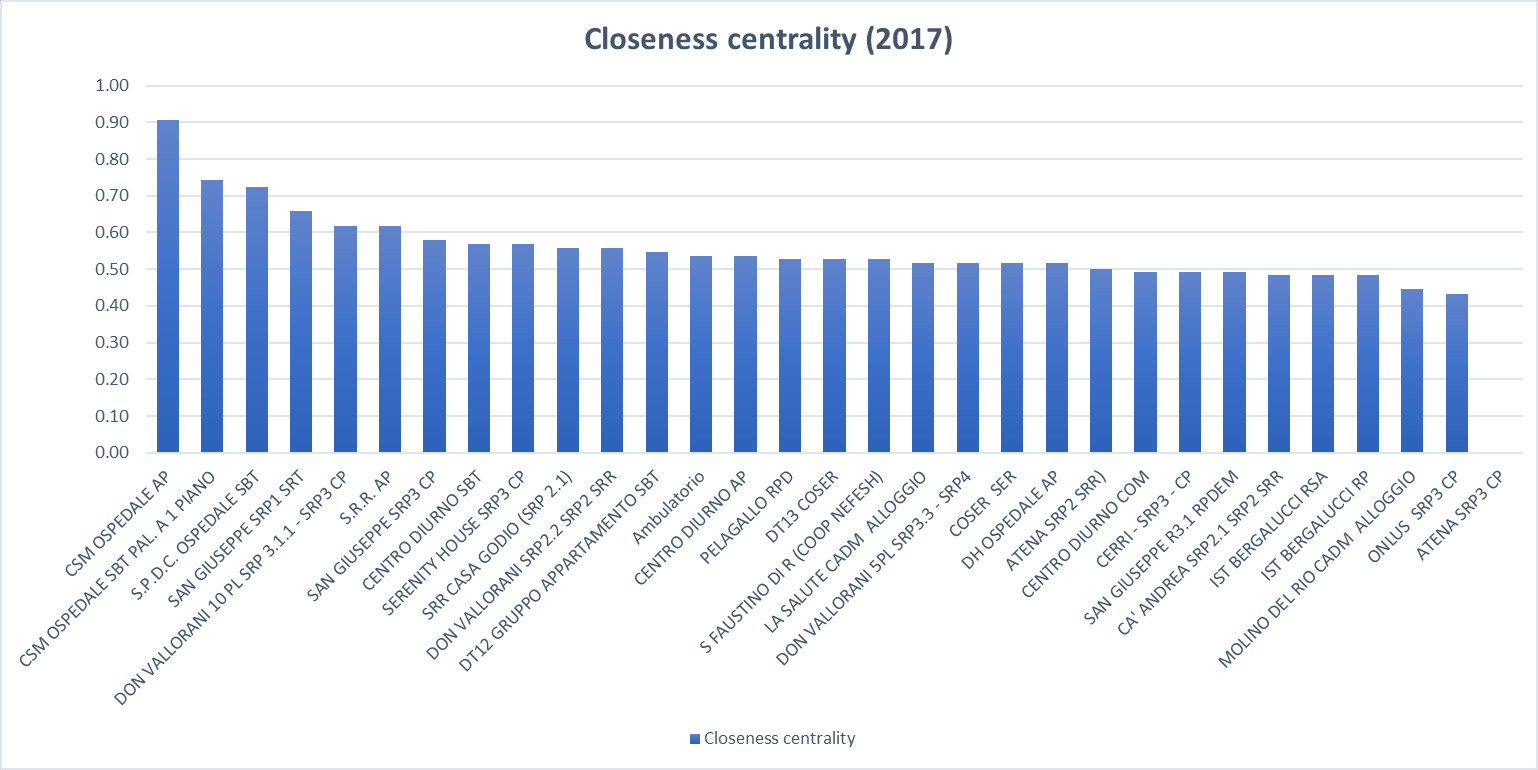
\includegraphics[width=0.8\linewidth]{imgs/2017_diagram}
		\label{fig:2017diagram}
	\end{figure}
\end{frame}

\section{Anno 2019}
\begin{frame}
	\frametitle{Anno 2019}
	\framesubtitle{Statistiche generali}
	\begin{itemize}
		\item Rete formata da 31 nodi e 105 archi.
		\item Il nodo pi� centrale � "CSM Ospedale SBT (Pal.A 1� piano)".
		\item Centralizzazione del grafo: 0,52. 
		\item Unica componente connessa.
	\end{itemize} 
\end{frame}

\begin{frame}
	\frametitle{Anno 2019}
	\framesubtitle{Centralit�}
	\begin{figure}
		\centering
		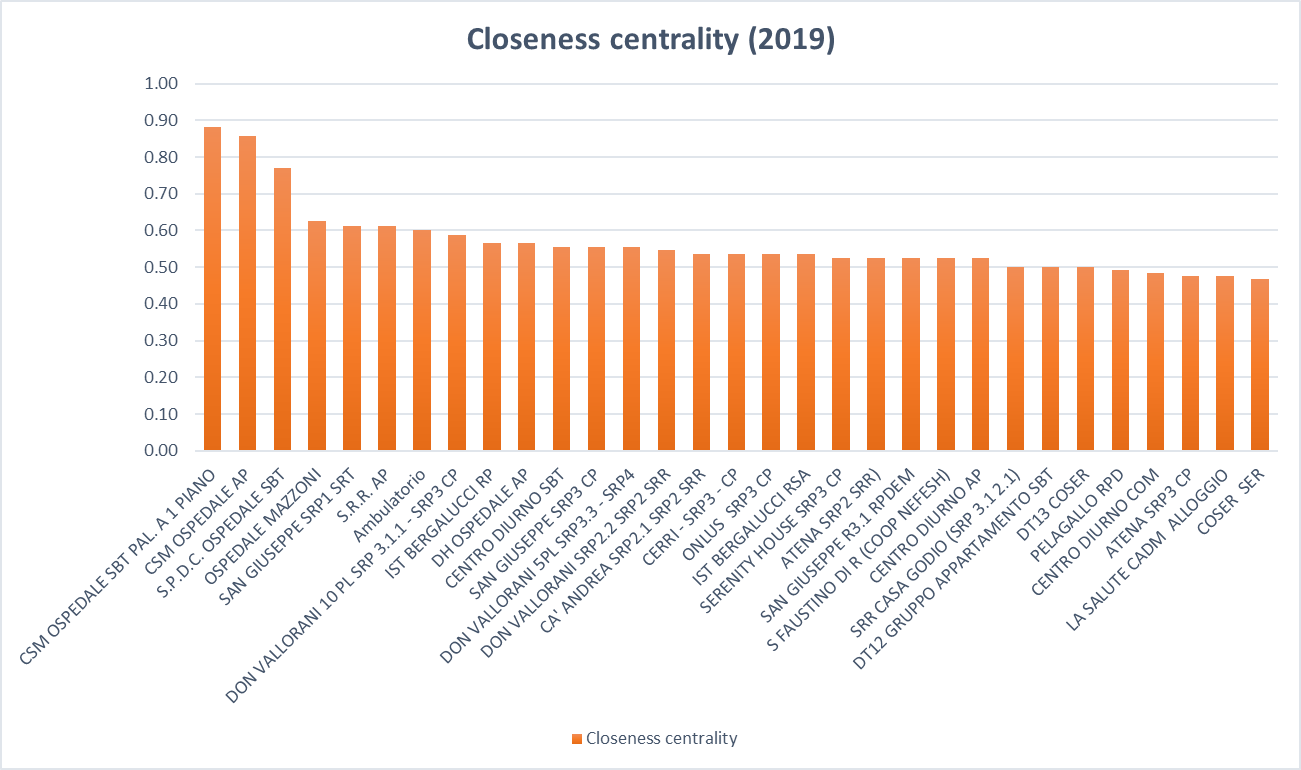
\includegraphics[width=0.8\linewidth]{imgs/2019_diagram}
		\label{fig:2019diagram}
	\end{figure}
\end{frame}



%============================== Eding document=====================================================
\end{document}




